\cleardoublepage
\chapter{Objetivos}
\label{chap:objetivos}


\section{Descripción del problema}
\label{sec:des_problema}


El problema al que se quiere dar una solución es la construcción de un sistema, que a partir de unas configuraciones de entrada, y cuya especificación sea trasladable al enunciado de las actividades prácticas de alumnos de asignaturas de programación de servicios y aplicaciones sobres redes de ordenadores, pueda proceder a su corrección requiriendo los mínimos cambios o ajustes en la implementación en dicho sistema.\\


Estas correcciones es deseable que puedan realizarse lo más desatendida y automáticamente posible, permitiendo liberar tiempo al profesor y disminuir el tiempo de respuestas, además de proporcionarles con poco retraso con respecto al día de entrega de un conjunto variado de información acerca de los resultados de sus prácticas con el objetivo de incidir positivamente en el aprendizaje tanto de los conceptos de la asignatura como de habilidades en programación.\\


Los elementos que debemos considerar en la corrección del alumno son los siguientes:\\

\begin{itemize}
\item En general, un repositorio Git, no ``bare'', en el cual el alumno ha estado trabajando y pueda observarse su evolución trabajando en la actividad, cuyo directorio de trabajo contenga los entregables predefinidos por la especificación o enunciado de la actividad.\\

\item Ficheros de código fuente: trabajando casi siempre con fuentes en Python 2 o 3.\\

\item Capturas de Wireshark: dado que estamos evaluando a alumnos que cursan asignaturas relacionadas con servicios o aplicaciones lanzadas sobre redes, es un tipo de entregable muy útil para evaluar el funcionamiento de programas cliente o servidor que se entregan.\\

\item Otros ficheros de texto o XML, cuya inclusión venga justificada por contener configuraciones o datos de entrada para los \textit{scripts}, o sean en sí mismo uno de los entregables evaluables, como por ejemplo una actividad acerca del lenguaje SMIL, que es una especificación XML.\\
\end{itemize}


En base a esos entregables, tenemos que plantearnos el sistema automatizado, que nos ayude a evaluar con el mayor grado de detalle posible que la actividad ha sido entregada completamente en los términos especificados por el enunciado y la funcionalidad se cumple, demostrando el aprovechamiento de la actividad.


\section{Punto de partida}
\label{sec:puntp_partida}


Para la realización de este sistema, no se parte de cero. Ya que fruto de las nuevas experiencias docentes introducidas por el profesor, éste desarrolló unos \textit{scripts} semiautomáticos para poder agilizar la corrección y disponer los alumnos de sus reportes antes de la siguiente sesión práctica.\\


Aunque estos \textit{scripts} todavía exigen bastante intervención manual , es una muy buena primera aproximación y permite abordar todo el proceso de corrección que de otra forma llevaría días o semanas, y sin tanta cantidad de información y resultados susceptibles de evaluar y poder incidir sobre ellos en las clases.\\

\begin{figure}[H]
   \centering
   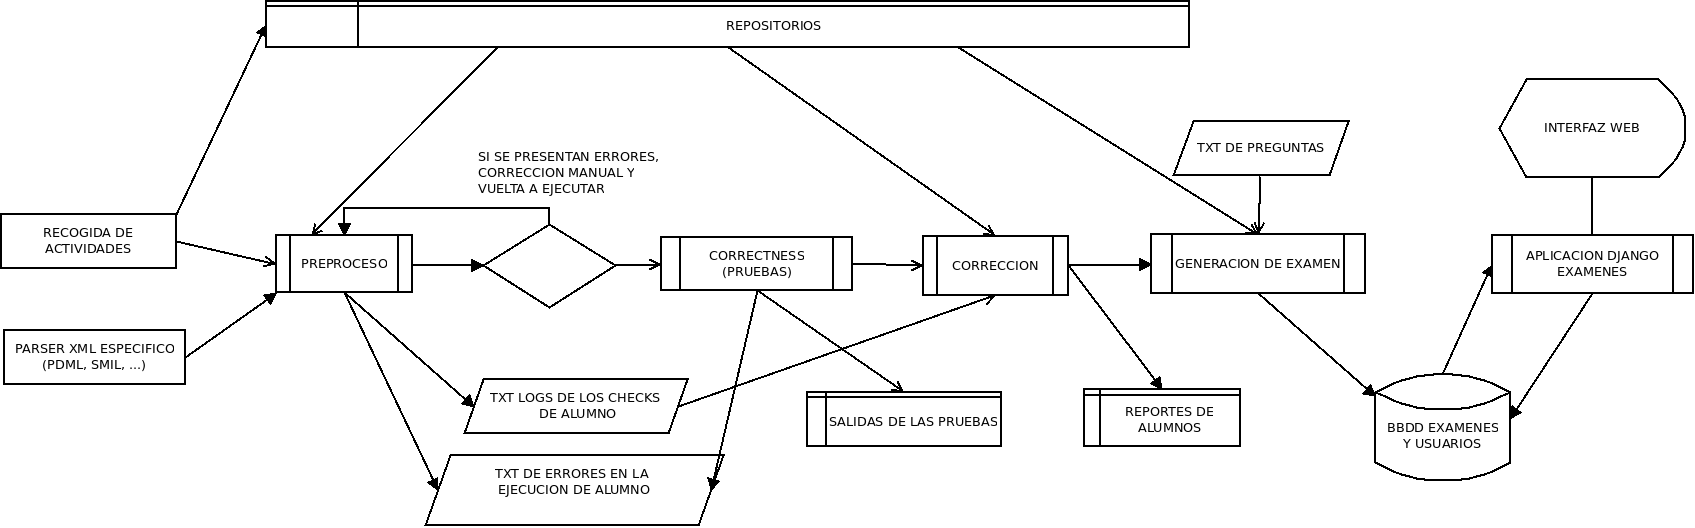
\includegraphics[width=16cm, height=7cm]{img/Diagram1_flujo_semiautomatico}
   \caption{Flujo de los scripts semiautomáticos de la experiencia piloto}
   \label{figura:flujo_semiautomatico}
\end{figure}


Según algunos reportes del profesor, con esta metodología, se podía evaluar una actividad en una mañana o una jornada, según la complejidad particular de las correcciones, y teniendo en cuenta muchos más información disponible para evaluar que otras formas de evaluación prácticas habituales en asignaturas similares.\\


Este sistema de \textit{scripts}, que se introduce en la figura anexa, se compone de los siguientes procesos, la mayoría de ellos implementados por un módulo o script Python.\\


\subsection{Recuperación de los datos}
\label{sec:rec_datos}


En general es un proceso aparte de los \textit{scripts} planteados. Cuando yo realicé estas experiencias, consistía en que los administradores de los laboratorios de la universidad automáticamente recopilaban las rutas de entrega que se habían especificado dentro del \textit{home} de cada alumno.\\


Actualmente, se solicita el usuario público de los alumnos en el servicio Github, donde se especifica que inicien un repositorio con el nombre especificado para realizar la entrega, para configurarlos en el preproceso y clonarlos.\\



\subsection{Preproceso}
\label{sec:preproceso}


En este módulo se lee y establece la configuración inicial con las especificaciones de la entrega tales como los usuarios de los alumnos, localización de repositorios, listado de ficheros a entregar, etc.\\


Una vez establecida la configuración. Se lanzan diferentes comprobaciones sobre los ficheros mediante funcionalidad python o invocando terceras utilidades con llamadas al sistema. La salida se vuelca a ficheros de texto en un formato parseable, y los errores en la ejecución de los ``checks'' a otro fichero de errores, que revisa el profesor por si tiene que tomar acciones correctoras sobre el repositorio afectado y ejecutar nuevamente los ``checks''.\\


\begin{itemize}
\item La existencia del listado de ficheros exigido.\\

\item Evaluación de errores de estilo en el código Python, con ayuda de pep8.\\

\item Evaluación de prácticas de mala calidad de código, con pylint.\\

\item Lectura del \textit{log} del repositorio Git, extrayendo el número de commits y su fecha.\\

\item En las actividades que lo exijan, ejecutar el módulo parser XML personalizado a la actividad para el chequeo de capturas Wireshark, convertidas a PDML, o la evaluación del contenido de las etiquetas y los atributos de cualquier otro fichero XML.
\end{itemize}


\subsection{Parseo XML: PDML, SMIL}
\label{sec:parseo}

La utilidad de este módulo sale a relucir en las entregas dónde los alumnos entregan capturas Wireshark con las trazas resultantes de ejecutar sus escenarios, las cuáles se convierten a PDML (ver las figuras inferiores) para facilitar su análisis. También en alguna otra actividad donde se han tratado con lenguajes XML, como el caso de SMIL.\\


\begin{figure}[H]
   \centering
   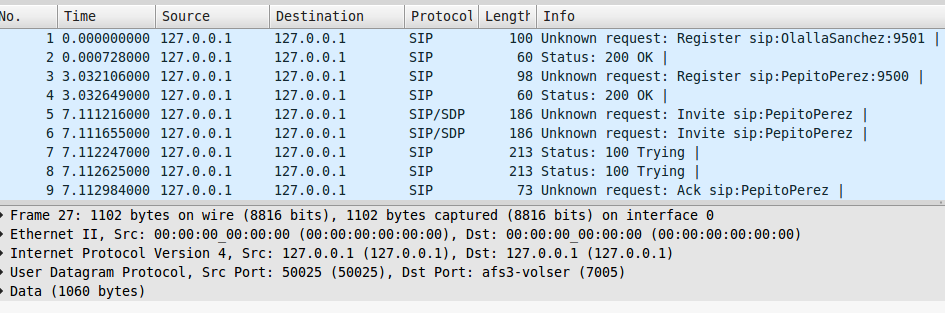
\includegraphics[width=16cm]{img/Selection_014_traza_wireshark}
   \caption{Traza de una captura de red visualizada}
   \label{figura:traza_wireshark}
\end{figure}


La aproximación que se sigue para el análisis, es utilizar el módulo SAX de Python para implementar específicamente para la actividad concreta que estamos corrigiendo, las comprobaciones sobre estos ficheros sobre las etiquetas, atributos o valores de ellas. Para demostrar que la traza o el XML ha sido generado o tiene los contenidos que se esperan, de haber realizado el alumno la tarea correctamente.\\


\begin{figure}[H]
   \centering
   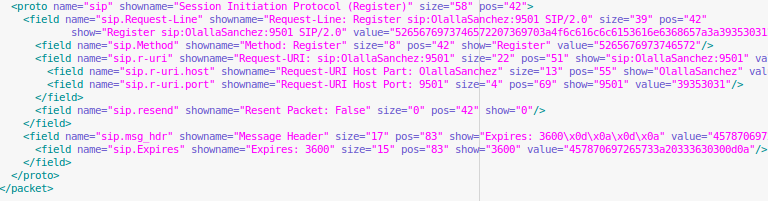
\includegraphics[width=16cm]{img/Selection_015_pdml_2}
   \caption{Extracto de un PDML de una trama SIP dentro la última capa de un paquete}
   \label{figura:extracto_pdml}
\end{figure}


Una vez el profesor ha implementado las comprobaciones en un módulo \textit{parser} específico, se invoca en el módulo de preproceso y se recogen los resultados impresos en el \textit{log} desde el módulo de corrección.


\subsection{Correctness}
\label{sec:correctness}


Correctness es el módulo de ejecución de pruebas de caja negra, se lanzan las llamadas sobre los \textit{scripts} de los alumnos para probar su funcionalidad ante determinadas entradas o ficheros de entrada, y se recogen los resultados y errores en los \textit{logs}.\\


Estas salidas se pueden comparar en el posproceso con el resultado esperado por el procesor, en el caso de actividades más sencillas o aquellas que se defina en el enunciado un formato de salida muy estricto. En caso contrario, la salida se almacena dentro del pool de ficheros de reporte del alumno para la posterior inspección del profesor.\\


\subsection{Posproceso}
\label{sec:posproceso}


La funcionalidad de este \textit{script} es parsear los logs del preproceso con el resultado de los ``checks'' y , generando un reporte en formato texto con el detalle sobre el resultado de las comprobaciones realizadas y su resultado, y el desglose de sus errores de estilo y avisos sobre líneas de código que incurren en algún uso del código no considerado de calidad según lo generalmente aceptado. Según el caso, también el resultado de las pruebas de caja negra.


\subsection{Generación de examen}
\label{sec:gen_exam}

En este script, se inyecta a una base de datos SQL, asociada también a una aplicación Django, las preguntas de la prueba que se hace a los alumnos para evaluar si el alumno conoce su propio código y cuestiones que evaluen.\\


Estas preguntas se inyectan de dos fuentes. La primera viene desde los propios ficheros fuente de la entrega, para la cual se inyecta un fragmento de ćodigo y se pregunta a cuál de los ficheros fuente pertenece.\\


La segunda fuente, es un fichero de texto, parseable, donde el profesor formula preguntas acerca de conceptos aplicados en la actividad, o cuestiones donde se le pide al alumno que indique cuál es la salida o que cambio tiene que hacer en un fragmento de código indicado.\\

\begin{figure}[H]
   \centering
   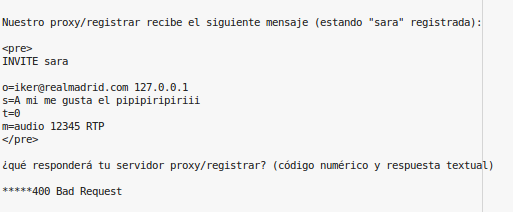
\includegraphics[width=16cm]{img/Selection_020_expregunta}
   \caption{Formato de la pregunta de examen que se sube a la BBDD}
   \label{figura:formato_examen}
\end{figure}



\subsection{Detección de plagio}
\label{sec:detec_plagio}


Esta tarea no está integrada dentro del resto de scripts, pero también forma parte del proceso de corrección, especialmente en las últimas entregas de las diferentes asignaturas.\\


En este paso del proceso de corrección, se suben las rutas con los códigos al servidor de la herramienta MOSS, donde se realiza el análisis y pasado un tiempo devuelven.\\


MOSS mide la similitud de entre ficheros texto a través de métodos estadísticos y establece esta medida fichero a fichero. Según el tipo y no es un hecho fuera de lo habitual encontrarse ante falsos positivos, especialmente si usamos MOSS para cotejar los códigos de las actividades más simples.\\

\begin{figure}[H]
   \centering
   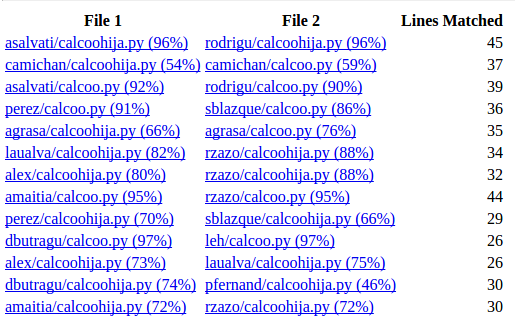
\includegraphics[width=16cm]{img/Selection_021_moss}
   \caption{Resultado que publica MOSS en una url}
   \label{figura:res_moss}
\end{figure}

\section{Requisitos}
\label{sec:requisitos}


Una vez estudiado todo el escenario de nuestro problema y la funcionalidad semiautomática de los \textit{scripts} de corrección, se estuvo definiendo de forma general entre proyectando y tutor algunos de los requisitos que se extrajeron de este análisis, obteniendo así el siguiente listado de requisitos a tener en cuenta en el sistema Misture:

\begin{itemize}
\item Análisis de qué ficheros han sido entregados en el repositorio, mejorando la experiencia del \textit{script}, limitada a verificar un listado inicial de ficheros.\\

\item Solucionar el caso frecuente de pequeñas desviaciones en los nombres de fichero.\\

\item Identificación del tipo de código de una fuente o el tipo del fichero, y algunos 	parámetros adicionales como la cantidad de líneas de código.\\

\item Análisis de la estructura de los códigos Python ampliado.\\

\item Incrementar la funcionalidad inicial que se limitaba a contar las clausulas ``class'' o ``def'' en los ficheros Python determinados inicialmente.\\

\item Análisis de errores de estilo, y calidad de código. Los pilotos cuentan la cantidad de errores de estilo de pep8 y de warnings sobre un análisis estático del código de pylint y reportan al profesor un resumen en formato texto de la cantidad de errores por tipo.\\

\item Enriquecer la funcionalidad del análisis Git, hasta ahora basado en el análisis del \textit{log} del repositorio, contando la cantidad de commits y la marca de tiempo entre primer y último commit.\\

\item Ampliar la funcionalidad del tratamiento de las capturas Wireshark, aprovechando todas las posibilidades que permite la conversión a PDML.\\

\item Como un plus, plantear, de ser posible, una utilidad de antiplagio libre como sustitutiva a MOSS.\\
\end{itemize}


\section{Objetivos generales}
\label{sec:obj_gen}


Una vez descrito el problema con el que estamos tratando, partiendo de la base de las experiencias piloto con la parte práctica de las materias, podemos establecer cuál es el objetivo.\\


El objetivo principal de Misture, es la integración de un conjunto de utilidades y de diferentes comprobaciones y pruebas de diferente índole, que van a enfrentarse contra el conjunto códigos fuentes y ficheros entregables que los alumnos generan en las diferentes actividades.\\


Esta integración debe buscar que el proceso sea lo más parecido a un flujo automatizado que reduzca el tiempo empleado por el corrector, que le permita centrarse en aquellas subtareas de una corrección donde más pueda aportar.\\


Por ejemplo, el profesor en base a estadísticas del análisis y a indagar a partir de ellos, puede detectar ciertos hábitos o malas prácticas desarrollando o aplicando los conceptos teóricos de la asignatura, o decidir dar una clase de refuerzo, enseñar cierta práctica o patrón de diseño, etc. Y esto es más valioso para todos que si tuviera que centrarse más bien en chequear entrega a entrega si un alumno ha escrito más o menos funciones, de más o menos longitud o complejidad, si su forma de escribir código es poco clara, etc.\\


Asimismo, el objetivo incluye un tratamiento más organizado de la información extraída, por ejemplo en BBDD, y la posibilidad de poder ofrecer un reporte más rico, sencillo, y fácil de ampliar o modificar frente al tratamiento que ofrecen los ficheros txt, que contienen las salidas heterogéneas de las diferentes utilidades y pruebas.\\


Para la consecución de dicho objetivo, tenemos como punto de partida el conjunto de scripts semiautomáticos que nos ha proporcionado el tutor utilizadas para las experiencias piloto, junto al reporte de incidencias u observaciones realizadas durante la ejecución y realización de alguna corrección, para intentar buscar mejoras en las funcionalidades que permitan reducir los puntos críticos en la corrección, que incapacitan la acción del \textit{script} y llevan a una revisión manual por parte del tutor. \\


\section{Objetivos Específicos}
\label{sec:obj_esp}


Aunque ya definidos los requisitos funcionales generales que exige el problema, y los objetivos generales. De estos podemos derivar algunos y concluir otros complementarios, que no debemos perder de vista para la consecución del objetivo general:\\


\begin{itemize}
\item Establecer el proyecto Python, que recogiera las funciones básicas, detectadas en las muestras de las actividades entregables de las asignaturas de programación de aplicaciones y servicios Web y multimedia en redes, adaptada a las características de las pequeñas prácticas realizadas por los alumnos.\\

\item Encontrar los mecanismos necesarios, para automatizar al máximo cada una de las funcionalidades básicas, reduciendo al mínimo la cantidad de pasos o funcionalidades semiautomáticas o manuales llevabas a cabo habitualmente por el profesor en las experiencias piloto descritas.\\

\item Como en nuestro contexto nos hallamos ante alumnos en proceso de aprendizaje de destrezas de programación. Se debe buscar el permitir cierta tolerancia en la automatización a errores por parte de los alumnos en los códigos o en los ficheros entregables.\\


Este objetivo puede en muchos casos añadir complejidad a la resolución de nuestros propósitos. Pero la detección y rectificación automatizada de estos redundaría en reducir las intervenciones manuales y re-ejecuciones de los \textit{scripts} de los diferentes pasos de la corrección.\\

\item En consecuencia a los anteriores, disminuir el tiempo dedicado por el docente en el desarrollo o adaptación del código para la corrección de nuevas actividades, su ejecución, y la recogida de resultados y reporte de los puntos críticos a revisar.\\

\item Mejora en la generación, riqueza, y comunicación del \textit{reporting} de los resultados de los diferentes análisis y correcciones que se ejecutan sobre los repositorios.\\

\item Mejorar la recogida de información extraída en las correcciones, de forma persistente y debidamente relacionada en sistemas de BBDD, permitiendo nuevos análisis posteriores, y ahorrando tiempo y re-ejecuciones en caso de errores que requieran alguna intervención manual por parte del profesor.\\

\item Interrelacionar nuestro sistema con una interfaz web, en una primera aproximación, para la realización de exámenes de verificación de autoría y conocimiento del código del alumno. Asimismo, mejorar la experiencia piloto de forma que se pueda extender la funcionalidad de la interfaz web a mostrar.\\

\item A título personal, con la realización de este proyecto, pretendía, en el momento de su elección, adquirir el conocimiento o destreza en diferentes áreas y tecnologías:\\

\begin{itemize}
\item Python 3, puesto que durante mi ciclo universitario la versión generalmente estudiada era Python 2.\\

\item MongoDB, cuyo paradigma de BBDD no había tenido la oportunidad tampoco de estudiar y practicar en ninguna asignatura.\\

\item Git, del cuál tenía un breve conocimiento básico – add, commit, pull, push – y empleado para usos individuales y no colaborativos.\\

\item Ampliar conocimientos sobre el análisis de código fuente, de repositorios, de fuentes de información heterogéneas.
\end{itemize}
\end{itemize}




